\documentclass{article}

\usepackage[utf8]{inputenc}  
\usepackage[T1]{fontenc}   
\usepackage{amsmath}
\usepackage{amsfonts}
\usepackage{pgfplots}
\usepackage{sagetex}
\usepackage{graphicx}
\usepackage{caption}
\usepackage{subcaption}
\usepackage{minted}

\usepackage{geometry}
\geometry{hmargin=1.5cm,vmargin=1.5cm}

\newcommand{\BigO}[1]{\ensuremath{\operatorname{O}\left(#1\right)}}

\newcommand{\Deriv}[1]{\ensuremath{\frac{d}{dx}(#1)}}
\newcommand{\DDeriv}[1]{\ensuremath{\frac{d#1}{dx}}}
\newcommand{\SmallO}[1]{\ensuremath{\operatorname{o}\left(#1\right)}}

\newcommand{\BBigO}[3]{\ensuremath{\underset{#1 \to #2 }{\operatorname{O}\left(#3\right)}}}
\newcommand{\BigF}[2]{\ensuremath{#1 \left(#2\right)}}
\newcommand{\Wrap}[1]{\ensuremath{\left(#1\right)}}
\newcommand{\Q}[1]{\subsubsection*{Question #1}}

\begin{document}

\title{MAP431 - Projet}
\author{BIAD Anas / EL KHADIR Bachir}


\maketitle

\Q{1} 

Soit $ v \in H_{0}^{1}(\Omega) $ \\
On multiplie l'équation par la fonction test $v$ et on intègre par parties en utilisant la formule de Green : 
\begin{align*} 
 \int_{\Omega}  f(x)v(x)dx   &=  \int_{\Omega}  v(x)u_{\mu}(x)dx   -  \int_{\Omega}  \Deriv{ \kappa_{\mu}(x) \DDeriv{u_{\mu}}(x) } v(x)dx  \\
&= \int_{\Omega}  v(x)u_{\mu}(x)dx  +  \int_{\Omega}  \kappa_{\mu}(x) \DDeriv{v}(x) \DDeriv{u_{\mu}}(x) dx \\
\end{align*}
\\
Donc la forumation variationnelle du problème (3) s'écrit : 
$$a_{\mu}(u_{\mu},v) = b(v)$$ 
où : 
$$a_{\mu}(u_{\mu},v) = \int_{\Omega}  v(x)u_{\mu}(x)dx  +   \int_{\Omega}  \kappa_{\mu}(x) \DDeriv{v}(x) \DDeriv{u_{\mu}}(x) dx $$ 
$$b(v) =  \int_{\Omega}  f(x)v(x)dx $$

% -------------------------------------------- QUESTION 2 --------------------------------------------
\Q{2}

Les coefficients de A:
\begin{align*}
A_{i,j} = a_{\mu}(\varphi_{i},\varphi_{j}) =
\left\{\begin{array}{ll}
\frac{2}{h^{2}} \int_{K_{i}} \kappa_{\mu}(x) dx + \frac{2}{3}h & \mbox{si} \, i = j \\
-\frac{1}{h^{2}} \int_{K_{i}} \kappa_{\mu}(x) dx + \frac{h}{4} & \mbox{si} \, j = i+1 \\
-\frac{1}{h^{2}} \int_{K_{i-1}} \kappa_{\mu}(x) dx + \frac{h}{4} & \mbox{si} \, j = i-1 \\
0 & \mbox{sinon} \\
\end{array}
\right.
\end{align*}

Les coefficients de B:
\begin{align*}
B_i = b(\varphi_{i}) &= \int_{0}^{1} \varphi_{i}(x) sin(2\pi x)dx  \\
&= \int_{0}^{1} \varphi(\frac{x-x_{i}}{h}) sin(2\pi x)dx \\
&= h \, sin(2 \pi x_{i}) \,  (sinc(\pi h))^{2}
\end{align*}


%---------------------------------------   QUESTION 3 --------------------------------
\Q{3}
\subsubsection*{Le fichier calcul.sce contenant les fonctions calculant A, B puis la solution X}
\inputminted{scilab}{codes/calcul.sce}

\subsubsection*{Le fichier question3.sce qui calcule et affiche le résultat pour $\mu \in \{0.01, 0.1, 1\}$}
\inputminted{scilab}{codes/question3.sce}

\subsubsection*{Le résultat graphique}

\begin{figure}
\centering
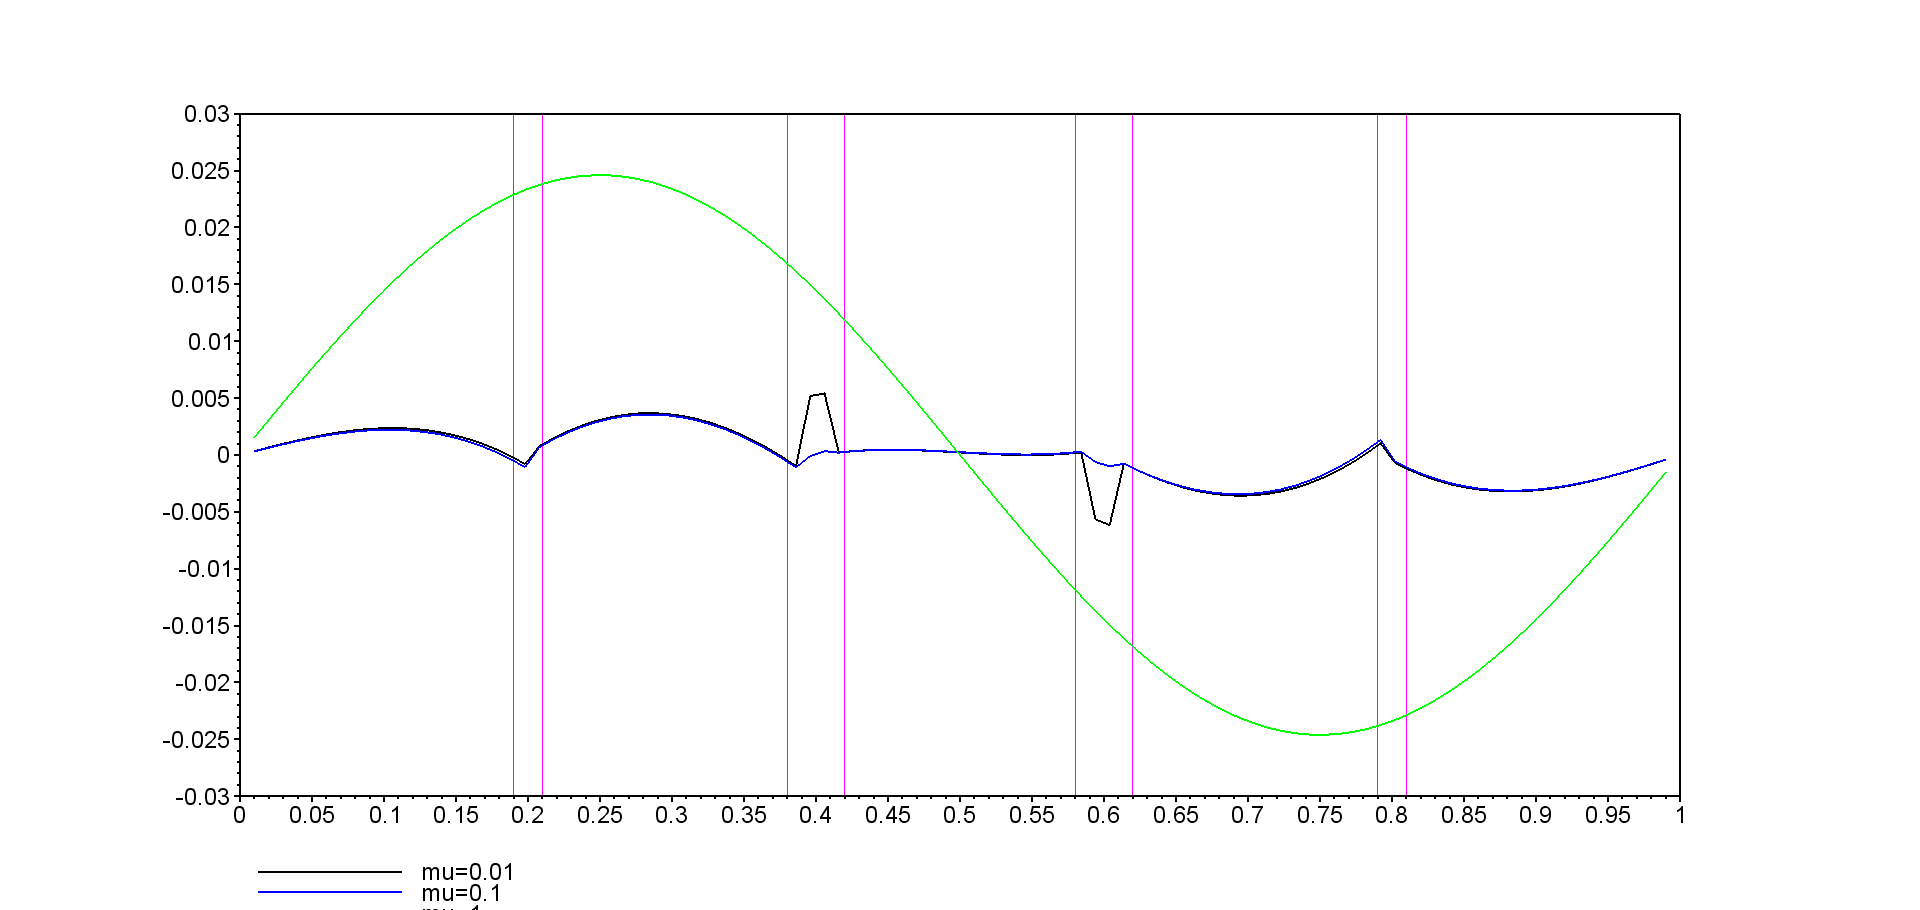
\includegraphics[scale=0.25]{img/q3.png}
\caption{courbe de $u_\mu$ pour $\mu \in \{0.01, 0.1, 1\}$}
\end{figure}


\subsubsection*{Commentaire}
commenatire ici

% ---------------------------------------   QUESTION 4 --------------------------------------------
\Q{4}
En injectant la relation:
$$ u_{\mu}^{RB} = \sum_{j=1}^{N_{0}} X_{\mu , j }^{RB} u_{j} $$ 
Dans:
$$ a_{\mu}( u_{\mu}^{RB} , u_{i} ) = b(u_{i}) $$ et 
On trouve : 
$$ \sum_{j=1}^{N_{0}} X_{\mu , j }^{RB} a_{\mu}(u_{j},u_{i}) = b(u_{i}) $$ 

Ainsi $ X_{\mu}^{RB} $ est solution du système linéaire : 
$$ A_{\mu}^{RB}X_{\mu}^{RB} = B^{RB} $$ 
Avec : 
$$ (A_{\mu}^{RB})_{i,j} = a_{\mu}(u_{j},u_{i}) $$
et : 
$$ (B^{RB})_{i} = b(u_{i}) $$

On a : 
\begin{itemize}
	\item $a_{\mu}$ est symétrique 
	\item $a_\mu$ est positive car $(\forall v \in H^0_1(\Omega)) \, a_{\mu}(v,v) = \int_{\Omega}  (v(x))^{2}dx  +   \int_{\Omega}  \kappa_{\mu}(x) (\DDeriv{v}(x))^{2}  dx >= 0$ 
	\item Si $  a_{\mu}(v,v) = 0 $ alors $ \int_{\Omega}  (v(x))^{2}dx = 0 $ , donc $v=0$ . Ainsi $ a_{\mu} $ est définie 
\end{itemize}
$ A_{\mu}^{RB} $ est la matrice de $a_\mu$ dans la base des $u_i$, donc $ A_{\mu}^{RB} $ est symétrique , définie positive.


%--------------------- ----------------------   QUESTION 5 ----------------------------------------
\Q{5}
on a : 
\begin{align*}
(A_{\mu})_{i,j} &= a_{\mu}(u_{\mu},v) \\
&= \int_{\Omega}  \varphi_i(x) \varphi_j(x)dx  +   \int_{\Omega_{1}} \DDeriv{\varphi_i}(x) \DDeriv{\varphi_j}(x) dx  +  \mu \int_{\Omega_{2}} \DDeriv{\varphi_i}(x) \DDeriv{\varphi_j}(x) dx \\
&= \int_{\Omega} \varphi_{j}(x) \varphi_{i}(x)dx  +   \int_{\Omega_{1}} \DDeriv{\varphi_{j}}(x) \DDeriv{\varphi_{i}}(x) dx 
+ \int_{\Omega_{2}} \DDeriv{\varphi_{j}}(x) \DDeriv{\varphi_{i}}(x) dx \\
&= (A_{0})_{i,j} + (A_{1})_{i,j}
\end{align*}
Où l'on a posé:
$$ A_{0} = \left(\int_{\Omega} \varphi_{j}(x) \varphi_{i}(x)dx  +   \int_{\Omega_{1}} \DDeriv{\varphi_{j}}(x) \DDeriv{\varphi_{i}}(x) dx\right)_{i, j} $$
$$ A_{1} = \left(\int_{\Omega_{2}} \DDeriv{\varphi_{j}}(x) \DDeriv{\varphi_{i}}(x) dx\right)_{i, j} $$
Et donc on a: $$ A_{\mu} = A_{0} + \mu A_{1} $$


D'autre part , on a 
\begin{align*}
(A_{\mu}^{RB})_{i,j} &= a_{\mu}(u_{j},u_{i}) \\
&= [u_{i}]_{(\varphi_{1},...,\varphi_{N})}^T \, A_\mu \, [u_{j}]_{(\varphi_{1},..,\varphi_{N})} \\
&= X_i^T A_\mu X_j \\
&= X_i^T A_0 X_j + \mu X_i^T A_1 X_j \\
&= (A_0^{RB})_{i,j} + \mu (A_1^{RB})_{i,j}
\end{align*}
et :
$$ (B^{RB})_{i} = b(u_{i}) = B^T X_i $$


%--------------------------------------------- QUESTION 6 ----------------------------
\Q{6}
\inputminted{scilab}{codes/calcul2.sce}
\inputminted{scilab}{codes/question6.sce}

Graphie ici
Commentaire ici

%---------------------------------------------   QUESTION 7 -----------------------
\Q{7}
\inputminted{scilab}{codes/question7.sce}
Graphie ici
Commentaire ici

%---------------------------------------------   QUESTION 8 -----------------------
\Q{8}
\inputminted{scilab}{codes/equation.edp}


\end{document}